\documentclass[12pt, letterpaper, twoside]{article}
\usepackage[utf8]{inputenc}
\usepackage[spanish]{babel}
\usepackage{amsmath, amsfonts, amssymb, amsthm}
\usepackage[left = 2cm, right = 2cm, top = 2cm, bottom = 2cm]{geometry}

\title{Grafos}

%Estilo de la página
\usepackage{fancybox, fancyhdr}
\pagestyle{fancy}
\fancyhf{}
\fancyhead[LE,RO]{\small{\leftmark}}
\fancyfoot[CE,CO]{\thepage}
\renewcommand{\headrulewidth}{2 pt}

%Imagenes
\usepackage{graphicx}
\graphicspath{{Imagenes/}}

%Estilo del codigo
\usepackage{listings}
\usepackage[dvipsnames]{xcolor}
\lstset{  
	language         = C++, 
	xleftmargin      = 1 cm,
	numbers          = left,
	numberstyle      = \tiny\textbf,	
	basicstyle       = \footnotesize,
	keywordstyle     = \color{blue},
	directivestyle   = \color{Green},
	commentstyle     = \color{purple},
	stringstyle      = \color{blue},
	showstringspaces = false,
	breaklines       = true,
}

%Documento
\begin{document}

\section{Caminos más cortos.}

Consideremos un grafo $G = (V, E)$ donde cada arista $(u, v)$ tiene una longitud $d(u,v) > 0$. El camino más corto entre dos vértices minimiza la longitud total del camino.

%$$-\dfrac{\frac{2\sin\left(\frac{{\pi}}{9}\right)\left(\sin\left(\frac{{\pi}}{9}\right)x-6\right)-2\sin\left(\frac{{\pi}}{9}\right)\left(31-\sin\left(\frac{{\pi}}{9}\right)x\right)+4\cos\left(\frac{{\pi}}{9}\right)\left(\cos\left(\frac{{\pi}}{9}\right)x+9\right)}{2\sqrt{\left(31-\sin\left(\frac{{\pi}}{9}\right)x\right)^2+\left(\cos\left(\frac{{\pi}}{9}\right)+9\right)^2}\sqrt{\left(\sin\left(\frac{{\pi}}{9}\right)x-6\right)^2+\left(\cos\left(\frac{{\pi}}{9}\right)+9\right)^2}}+\frac{\sin\left(\frac{{\pi}}{9}\right)\left(31-\sin\left(\frac{{\pi}}{9}\right)x\right)\left(\left(\sin\left(\frac{{\pi}}{9}\right)x-6\right)^2+\left(31-\sin\left(\frac{{\pi}}{9}\right)x\right)^2+2\left(\cos\left(\frac{{\pi}}{9}\right)x+9\right)^2\right)}{2\left(\left(31-\sin\left(\frac{{\pi}}{9}\right)x\right)^2+\left(\cos\left(\frac{{\pi}}{9}\right)+9\right)^2\right)^\frac{3}{2}\sqrt{\left(\sin\left(\frac{{\pi}}{9}\right)x-6\right)^2+\left(\cos\left(\frac{{\pi}}{9}\right)+9\right)^2}}-\frac{\sin\left(\frac{{\pi}}{9}\right)\left(\sin\left(\frac{{\pi}}{9}\right)x-6\right)\left(\left(\sin\left(\frac{{\pi}}{9}\right)x-6\right)^2+\left(31-\sin\left(\frac{{\pi}}{9}\right)x\right)^2+2\left(\cos\left(\frac{{\pi}}{9}\right)x+9\right)^2\right)}{2\sqrt{\left(31-\sin\left(\frac{{\pi}}{9}\right)x\right)^2+\left(\cos\left(\frac{{\pi}}{9}\right)+9\right)^2}\left(\left(\sin\left(\frac{{\pi}}{9}\right)x-6\right)^2+\left(\cos\left(\frac{{\pi}}{9}\right)+9\right)^2\right)^\frac{3}{2}}}{\sqrt{1-\frac{\left(\left(\sin\left(\frac{{\pi}}{9}\right)x-6\right)^2+\left(31-\sin\left(\frac{{\pi}}{9}\right)x\right)^2+2\left(\cos\left(\frac{{\pi}}{9}\right)x+9\right)^2\right)^2}{4\left(\left(31-\sin\left(\frac{{\pi}}{9}\right)x\right)^2+\left(\cos\left(\frac{{\pi}}{9}\right)+9\right)^2\right)\left(\left(\sin\left(\frac{{\pi}}{9}\right)x-6\right)^2+\left(\cos\left(\frac{{\pi}}{9}\right)+9\right)^2\right)}}}$$
%\begin{center}
%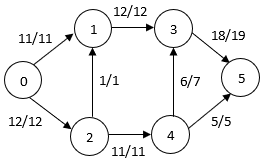
\includegraphics[width = 0.45\textwidth]{MaxFlow.png}	
%\end{center}

\subsection{Algoritmo de Dijkstra}

Complejidad: $O((|E| + |V|) \log|V|)$.

\lstinputlisting[firstline = 6]{Dijkstra.cpp} \medskip

\begin{tabular}{|p{7cm}|p{7cm}|}
	\hline
	\textbf{Entrada} & \textbf{Salida}\\ \hline
	6 8 & Flujo maximo: 23\\
	0 1 11 & 0 1: 11/11\\
	0 2 12 & 0 2: 12/12\\
	1 3 12 & 1 3: 12/12\\
	2 1 1  & 2 1: 1/1\\
	2 4 11 & 2 4: 11/11\\
	4 3 7  & 3 5: 18/19\\
	3 5 19 & 4 3: 6/7\\
	4 5 5 & 4 5: 5/5\\ 
	0 5 & \\ \hline
\end{tabular}

\newpage

\section{Máximo flujo.}

Consideremos un grafo dirigido $G = (V, E)$ donde cada arista $(u, v)$ tiene asociada una capacidad $c(u,v) > 0$. Un flujo de $s$ a $t$ es una función que a cada arista le asigna un número $f(u,v)$ que satisface
\begin{itemize}
\item $f(u, v) \leq c(u,v)$.
\item Para cualquier vértice $v \neq s, t$, el flujo que entra es igual al flujo que sale; $s$ solo tiene flujo saliente y $t$ solo tiene flujo entrante.
\end{itemize}
El flujo total es el flujo que sale de $s$.

%\begin{center}
%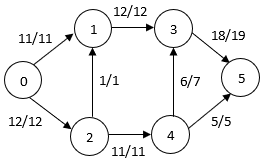
\includegraphics[width = 0.45\textwidth]{MaxFlow.png}	
%\end{center}

\subsection{Algoritmo de Edmonds-Karp}

Complejidad: $O(|V||E|^2)$.

\lstinputlisting[firstline = 6]{Edmonds-Karp.cpp} \medskip

\begin{tabular}{|p{7cm}|p{7cm}|}
\hline
\textbf{Entrada} & \textbf{Salida}\\ \hline
6 8 & Flujo maximo: 23\\
0 1 11 & 0 1: 11/11\\
0 2 12 & 0 2: 12/12\\
1 3 12 & 1 3: 12/12\\
2 1 1  & 2 1: 1/1\\
2 4 11 & 2 4: 11/11\\
4 3 7  & 3 5: 18/19\\
3 5 19 & 4 3: 6/7\\
4 5 5 & 4 5: 5/5\\ 
0 5 & \\ \hline
\end{tabular}

\newpage

\section{Emparejamiento máximo.}

Consideremos un grafo bipartito $G = (U \cup V, E)$. Un emparejamiento de $G$ es un subgrafo en donde cada vértice pertenece a lo más a una arista.

%\begin{center}
%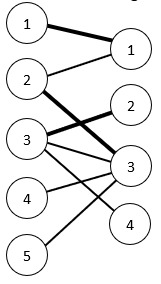
\includegraphics[height = 0.3\textheight]{MaxMatching.png}	
%\end{center}

\subsection{Algoritmo de Hopcroft-Karp}

Complejidad: $O(|E|\sqrt{|V|})$.

\lstinputlisting[firstline = 7]{Hopcroft-Karp.cpp} \medskip

\begin{tabular}{|p{7cm}|p{7cm}|}
\hline
\textbf{Entrada} & \textbf{Salida}\\ \hline
5 4 8 & Emparejamiento: 3\\
1 1   & 1 - 1\\
2 1   & 2 - 3\\
2 3   & 3 - 2\\
3 2   & \\
3 3   & \\
3 4   & \\
4 3   & \\
5 3   & \\ \hline
\end{tabular}

\end{document}